% typeset: Pdftex
% Afterwards compile with pdflatex > bibtex > pdflatex > pdflatex.
% in TeXShop preferences, changed edit from bibtex to biber
% beamer likes biber
% latex likes bibtex

% https://tex.stackexchange.com/questions/270633/beamer-and-the-pause-command
% https://tex.stackexchange.com/questions/1423/is-there-a-nice-way-to-compile-a-beamer-presentation-without-the-pauses
%\documentclass[handout]{beamer}
% https://tex.stackexchange.com/tags/accents/info
%
\documentclass[]{beamer}
\usepackage{pifont}
\newcommand{\cmark}{\text{\ding{51}}}
\newcommand{\xmark}{\text{\ding{55}}}
\usepackage{transparent}
\usepackage{epstopdf} % Automatic EPS to PDF conversion
% Fetch home directory
\usepackage{url}
\usepackage{tikz}
\usepackage{pgfplots}
\pgfplotsset{compat=1.17} % Ensure compatibility with PGFPlots
\usepackage{catchfile}
\CatchFileDef{\HomePath}{|kpsewhich -var-value=HOME}{}

% Strip trailing spaces from HomePath
\makeatletter
\edef\HomePath{\expandafter\zap@space\HomePath \@empty}
\makeatother

% Define base paths
% relies on symlink  at $HOME, e.g.
% 	GitHub -> /Users/dantopa//repos-xiuhcoatal/github
\newcommand{\pGithub}			{\HomePath/GitHub/}
\newcommand{\pGithubSharing}	{\pGithub/sharing/}
\newcommand{\pGlobal}			{\pGithubSharing/global/}
\newcommand{\pGlobalSetup}		{\pGlobal/setup-global/}
% Load Additional Setup Files
	% \input{\pGlobalSetup setup-global-beamer}

\input{\pGlobalSetup aesthetics-global.tex}
%\input{\pGlobalSetup beamer-beautify-hii.tex}
\input{\pGlobalSetup beautify-hii.tex}

\input{\pGlobalSetup paths-global.tex}
\input{\pGlobalSetup packages-global-beamer.tex}
\input{\pGlobalSetup math-global-beamer.tex}
\input{\pGlobalSetup hyperlinks-global.tex}
\input{\pGlobalSetup paths-bitbucket.tex}
\input{\pGlobalSetup libraries-global.tex}
\input{\pGlobalSetup macros-global.tex}

\input{\pGlobalSetup paths-local}

\endinput  %  -  -  -  -  -  -  -  -  -  -  -  -  -  -  -  -  -  -  -  -


	% \input{\pLocalSetup setup-local}

%\input{\pLocalSetup paths-local}
%\input{\pLocalSetup bibliography-local}
\input{\pLocalSetup hyperlinks-local}
%\input{\pLocalSetup input-libraries-local}

\input{\pLocalSetup macros-local}
% LaTeX macros to present a programming environment
% Looks like a terminal session, colored text on black background
\newcommand{\scru}[1]		{\bl   {\texttt{#1}}}
\newcommand{\scrk}[1]		{\bk   {\texttt{#1}}}
\newcommand{\scrg}[1]		{\gr   {\texttt{#1}}}
\newcommand{\scrr}[1]		{\rd   {\texttt{#1}}}
\newcommand{\scrv}[1]		{\dg   {\texttt{#1}}}
\newcommand{\scrz}[1]		{\mg   {\texttt{#1}}}
\newcommand{\scrc}[1]		{\textcolor{cyan}  {\texttt{#1}}}
\newcommand{\scrp}[1]		{\textcolor{purple}{\texttt{#1}}}
\newcommand{\scry}[1]		{\textcolor{yellow}{\texttt{#1}}}
\newcommand{\scrw}[1]		{\textcolor{white} {\texttt{#1}}}

%
\newcommand{\mySize}[1]		{{\normalsize{#1}}}
\newcommand{\myCanvas}[1]		{{\setbeamercolor{background canvas}{bg=black}{#1}}}
\newcommand{\myRasa}[1]		{\myCanvas{\mySize{#1}}}
\newcommand{\myFrame}[2]		{\myRasa{\begin{frame} \frametitle{#1} #2 \end{frame}}}
\newcommand{\myFoo}[2]			{\myFrame{#1}  \program \ \\[10pt] #2 \eprogram}


% tabs
%\newcommand{\tab}[0]     {\phantom{mm}}
\newcommand{\tab}[0]		{\ \ }
\newcommand{\spacer}[0]		{\ps\text{::}\ps}
\newcommand{\ps}[0]		{\phantom{m}}

% is equal?
\newcommand{\iseq}[0]		{ \overset{?}{=} }


\endinput  %  ==  ==  ==  ==  ==  ==  ==  ==  ==

% https://engineering.purdue.edu/ECN/Support/KB/Docs/LaTeXChangingTheFont
% \tiny
% \scriptsize
% \footnotesize
% \small
% \normalsize
% \large
% \Large
% \LARGE
% \huge
% \Huge% programming enviro

\endinput  %  ==  ==  ==  ==  ==  ==  ==  ==  ==


% Bibliography
	%\input{\pGlobalSetup packages-global-bibliography-charlie.tex}
\addbibresource{\pShareBibliographies/radar.bib} 

\newcommand{\fourier}		{\color{blue}{ e^{i n \theta} }} 

\setbeamercovered{transparent=10} % pause activated text
\usepackage{transparent}
\usepackage{seqsplit}
%\usepackage[T1]{fontenc}
%\usepackage[utf8]{inputenc}

\title[Input Slides 2024-12]{Input Slides 2024-12: My Two Slides}

\author[Daniel Topa]{\TopaHII \\ \TopaHIIEmail}
\institute{\missiontech} 
%\medskip

\date{\today}
%\date{2018-08-31}

\begin{document}

\begin{frame}
	\titlepage
\end{frame}
	%\include{\pSections "sec splash"}

\begin{frame}{Models of Satellite Cross Sections}
    \centering
    \begin{columns}[c,onlytextwidth]
        % Left Column: Satellite Image
        \begin{column}{0.4\textwidth}
            \centering
            % Light gray shading for the satellite
            \begin{tikzpicture}
                \node[inner sep=0pt] at (0,0) 
                {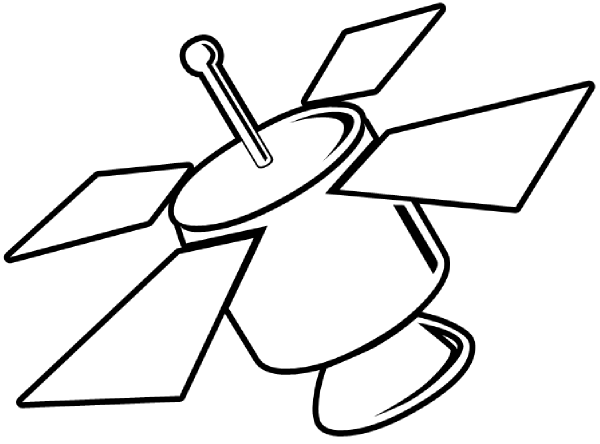
\includegraphics[width=0.9\linewidth]{\pLocalGraphics/satellites/satellite-outline-hi.png}};
                \fill[gray!10, opacity=0.5] (-1,0.5) rectangle (1,-1); % Light fill example
            \end{tikzpicture}
        \end{column}

        % Right Column: Spherical Harmonics Expansion
        \begin{column}{0.6\textwidth}
            \centering
            \textbf{\large Spherical Harmonics Expansion} \\[1em]
            \[
            f(r, \theta, \phi) \approx 
            \textcolor{blue}{a_{00}} Y_0^0 + \textcolor{blue}{a_{10}} Y_1^0 + \textcolor{blue}{a_{11}} Y_1^1 + \dots
            \]
        \end{column}
    \end{columns}

    % Bottom Line: Y_l^m Definition Spanning the Slide
    \vspace{1em}
    \textbf{where}
    \[
    Y_l^m (\theta, \phi) = \sqrt{\frac{(2l+1)(l-m)!}{4\pi (l+m)!}} P_l^m (\cos \theta) e^{i m \phi}
    \]
\end{frame}

\begin{frame}\frametitle{Overview}
	\tableofcontents[hideallsubsections]
\end{frame}

% main sections
	\input{\pSections "sec-writ-large"}
	\input{\pSections "sec-radiation"}
	\input{\pSections "sec-results"}
	%\input{\pSections "sec-mesh"}
	%\input{\pSections "sec-model"}
	%\input{\pSections "sec-software"}
	%\input{\pSections "sec-output"}
%\section{Bibliography}
%\begin{frame}[t,allowframebreaks]
%\frametitle{Bibliography}
%\nocite{strang}
%\printbibliography[heading=none]
%\end{frame}

{\tiny{
%\begin{frame}[allowframebreaks,shrink=10]\frametitle{Bibliography}
\begin{frame}[allowframebreaks]\frametitle{Bibliography}
	\nocite{*}
	\printbibliography
\end{frame}}}

% info slide during questions
\begin{frame}
	\titlepage
\end{frame}

\end{document}

%\tiny
%\scriptsize
%\footnotesize
%\small
%\normalsize
%\large
%\Large
%\LARGE
%\huge
%\Huge

%\, thin space (normally 1/6 of a quad);
%\> medium space (normally 2/9 of a quad);
%\; thick space (normally 5/18 of a quad);

\begin{frame}\frametitle{Frame Title}
\begin{enumerate}
	\item 
	\item 
	\item 
\end{enumerate}
\end{frame}

\begin{frame}\frametitle{Frame Title}
\begin{equation}
	\begin{array}{ccc} 
			%
			%
			%
	\end{array}
%\label{eq:}
\end{equation}
\end{frame}

\begin{frame}\frametitle{ }
\center
	\href{url}{
	\begin{overpic}[ scale = 1.0 ]
	{\pLocalGraphics graphic-file}
		%\put(-7,-10){Auxiliary text.}
	\end{overpic}}
\end{frame}

\begin{frame}\frametitle{Frame Title}
\begin{table}[htp]
%\caption{default}
\begin{center}
	\begin{tabular}{cc}
		%
		%
		%
	\end{tabular}
\end{center}
%\label{tab:label}
\end{table}%
\end{frame}

